\section{Drehstrom- Asynchronmaschinen (DAM)}
    \subsection{Aufbau der DAM}
        \begin{tabular}[c]{| p{3cm} | p{5cm} | p{4cm} | p{5cm} |}
            \hline
            Name &
            Aufbau &
            Positiv &
            Negativ \\
            \hline
            Schleifringläufer &
            Ständerwicklung und Läuferwicklung sind für Drehfelder gewickelt. Die Läuferwicklunganschlüsse sind rausgezogen, um einem Widerstand einzuschliessen. &
            Mit deiesem Widerstand lässt sich die Drehzahl regulieren &
            Die Schleifkontakte reduzieren den Wirkungsrad und erhöhen den Verschleiss. \\
            \hline
            Kurzschlussläufer / Käfigläufer &
            Die Läuferwicklungen sind immer kurzgeschlossen. &
            Es kann ein beinahge reibungsloser und verschleisfreier Betrieb ermöglicht werden &
            Die Drehzahl ist beinahe die Drehfeldfrequenz durch die Polzahl \\
            \hline
        \end{tabular}
    \subsection{Funktionsprizip}
        Das vom Ständer erzeugter Drehfeld erzeugt im stillstehenden, kurzgeschlossenen Läufer einen Drehstrom. Der Schlupf ist bei einem stillstehendem Läufer 1. Dieser Drehstrom erzeugt im Läufer ein Drehmoment. Dieses Drehmoment beschleunigt den Läufer.Durch verringert sich Schlupf, was wiederum ein kleineres Drehmoment nachsichtzieht. Bei einem Läufergeschwindigkeit, welche gelcih schnell ist wie das Drehfeld, reslutiert eine relative Geschwindigkeit von 0 (Schlupf von 0)$\rightarrow $ kein Drehmoment. Das heisst der DAM bewegt sich immer mit möglichst kleinem Schlupf.

    \subsection{Ersatzschaltbild}
        Da der DAM nach dem Induktionsgesetz funktionniert, kann man ihn gut als Trafo- Ersatzschaltbild darstellen. Der veränderliche Wirkwiderstand (Lastwiderstand) ist die mechanische Last. Das heisst die Verlustleistung über dem Widerstand ist die Mechanische Nutzleistung (minus die Reibungsverluste). Diese ist, wie man sieht von dem Schlupf abhnängig.
        \abb{images/ersatzschaltbild_DAM}{12cm}{Ersatzschaltbild des DAM mit Last}

     
     
    \subsection{Formeln zur Asynchronmaschine}
    \begin{tabular}[c]{ | p{6cm} | p{9cm} |}
    	\hline
    	Drehfeldzahl $[s^{-1}]$ bzw $[min^{-1}]$ & $n_d=\frac{f}{p}$ bzw
    	$n_d=\frac{f\cdot 60}{p}$\\
    	\hline
    	Schlupf $[-]$ & $s=\frac{n_d-n}{n_d}$\\
    	\hline
    	Zugeführte Wirkleistung & $P_{zu}= P_{el}=3\cdot U_1 \cdot I_1 \cdot
    	\cos\varphi$\\
    	\hline
    	Drehfeldleistung & $P_\delta=P_{el}-3\cdot\left(I_1^2\cdot R_1 +
    	P_{Fe}\right)=3\cdot\frac{R_2^\prime}{s}\cdot I_2^{\prime 2}$\\
    	\hline
    	Wellenleistung ohne Reibung & $P_{mech}=P_\delta-3I_2^{\prime 2}\cdot
    	R_2^\prime=(1-s)\cdot P_\delta$\\
    	\hline
    	Läuferverlustleistung & $P_{v2}=3\cdot R_2^\prime\cdot I_2^{\prime
    	2}=s\cdot P_\delta$\\
    	\hline
    	Drehmoment & $M=\frac{P_{mech}}{2\cdot\pi\cdot
    	n}=\frac{P_\delta}{2\cdot\pi\cdot n_0}$\\
    	\hline
    	Kippmoment & $M_{kipp}=\frac{3\cdot U_I^2}{4\pi\cdot
    	n_1}\cdot\frac{1-\sigma}{R_1(1-\sigma)+\sqrt{R_1^2+X_1^2}}\approx\frac{3\cdot
    	U_1^2}{4\pi\cdot n_1 \cdot X_\sigma}$\\
    	\hline
    	Klosssche Gleichung &
    	$\frac{M}{M_k}=\frac{2}{\left(\frac{s}{s_{kipp}}+\frac{s_{kipp}}{s}\right)}=\frac{2
    	s s_k}{s^2+s_k^2} $\\
    	\hline
    	Kippmoment Dreieckschaltung& $M_k= Faktor \cdot M_N$\\
    	\hline
    	für Sternschaltung & $M_{Stern}= \frac{M_\Delta}{3}$\\
    	\hline
    \end{tabular}
    
    \subsection{Drehmomentkennlinie}
        \begin{minipage}{5cm}
            \abb{images/Drehmomentkenn_DAM.png}{5cm}{$M = f(s)$}   
        \end{minipage}
        \begin{minipage}{13cm}
            $M_K = Kippmoment = Maximales Drehmoment$ \\
            $M_K \approx \frac{3 \cdot U_1^2}{4\cdot \pi \cdot n_1 \cdot X_\sigma}$ \\
            $X_\sigma = X_{\sigma 1} + X_{\sigma 1}^`$ \\
            $\frac{M}{M_K}\approx \frac{2}{\frac{s}{s_k}+\frac{s_k}{s}}$ \\
            $s_k = \frac{R_2^`}{\sqrt{R_1^2 + X_1^2}} \approx \frac{R_2^`}{X_\sigma}$    
        \end{minipage}
        \newpage

    \subsection{Ortskurve des DAM, Heyland- Kreis}
        \begin{minipage}{9cm}
            \abb{images/Heylandkreis.png}{8cm}{Heylandkreis mit Leistungs- und Momenteneinteilung}
        \end{minipage}
        \begin{minipage}{8cm}
            \abb{images/Heylandkreis_schlupf.png}{7cm}{Heylandkreis mit Schlupfskalierung}
        \end{minipage} \\
        \begin{minipage}{10.5cm}
            \begin{enumerate}     
                \item Den Massstab für den Strom wählen zB. $m_I=\frac{0.2 A}{mm}$
                \item Den Massstab für die Leistung berechnen: $P_{gesamt}=3U_N I_{Ph}$ $m_P=3U_N m_I$
                \item Den Massstab für das Drehmoment berechnen: $M=\frac{P_\delta}{2\pi n_0};$  $m_M= \frac{p\cdot m_P}{2\pi f}$  p = Polpaar
                \item $s=0 \rightarrow s_{0}$ messen und einzeichnen
                \item $s=1 \rightarrow s_{1}$ messen und einzeichnen
                \item Verlustleistung bei $s_{0}$ herauslesen ($P_{Fe}$) (ev. wenn nicht schon getan, mit \\ $P_{FE} = U \cdot I_{Wirk}$ den Leistungs-Massstab bestimmen.)\\
                \item $\perp$ vom Mittelpunkt von $\overline{s_{0}s_{1}}$
                \item Schnittpunkt auf $s_{0}- Achse (Richtung -j) = M$
                \item Kreis um M mit Schnittpunkt $s_{0}$ und $s_{1}$
                \item $I_N =$ Tangente auf dem Kreis vom Ursprung (0,0)
                \item $P_{v1}$ bei $s_{1}$ ausrechnen = $P_{R_1}$ von der Parallele zur J-Achse, welche durch M geht nach oben abtragen.
                \item Verbindung des Punktes zu $s_{0}$ verlängern $\rightarrow$ $s_{\infty}$
                \item \textit{ Bei Vereinfachung $R_{Cu}=0:\\ s_{0}$ auf Imaginär- Achse; $s_{\infty}$ auf Imaginär-Achse}
                \item Schlupf- Skalierung: $\perp$ auf $\overline{s_{\infty}M}$
                \item Schnittpunkt mit Verlängerung $\overline{s_{1}s_{\infty}}= 1$
                \item Schnittpunkt mit $\overline{s_{0}s_{\infty}}= 0$
                \item Dazwischen lineare Unterteilung
            \end{enumerate}
        \end{minipage}
        \begin{minipage}{7cm}
            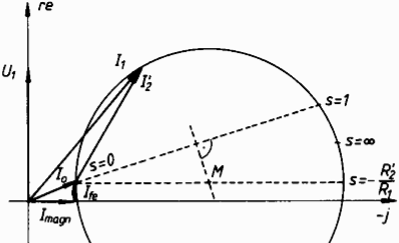
\includegraphics[width=6cm]{../ElMasch/images/StromortskurveDAM.png}\\
            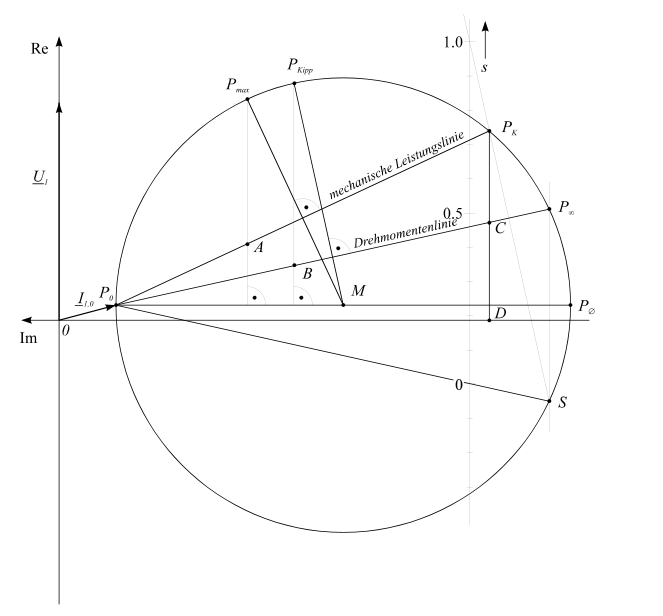
\includegraphics[width=8cm]{../ElMasch/images/OssannakreisPkipp.png}
        \end{minipage}
        \newpage
    \subsection{Orskurve des DAM, Heyland-Kreis 2. Anleitung}
    \begin{enumerate}
      \item Daten für Leerlauf und (echten) Kurzschluss der DAM verifizieren
      bzw. berechnen
      \item Massstäbe festlegen
      \begin{enumerate}
        \item Strommassstab $m_{I_{Ph}}$ Wählen bzw. Tipp befolgen
        \item Leistungsmassstab $m_{P_{gesamt}}=3U_{Ph}\cdot m_{I_{Ph}}$
        \item Drehmomentsmassstab $m_M=\frac{m_{P_{gesamt}}}{2\pi n_0} =
        \frac{m_{P_{gesamt}}\cdot p}{2\pi f}$
      \end{enumerate}
      \item Leerlaufpunkt $(s=0)$ aus $P_0$ und $I_0$ bestimmen und in die
      Grafik $U_{ph},-jI_{Ph}$ eintragen
      \item Anlaufpunkt $(s=0)$ aus $P_{KS}$ und $I_{KS}$ bestimmen und in die
      Grafik $U_{ph},-jI_{Ph}$ eintragen
      \item Mittelpunkt der Strecke (Anlaufpunkt-Leerlaufpunkt) bestimmen und
      Ossanakreis zeichnen
      \item Bremspunkt $s=\infty$ zeichnen je nach Aufgabenstellung
      \begin{enumerate}
        \item Anlaufmoment = lotrechte Strecke ausgehend vom Anlaufpunkt $(s=1)$
        \item Verluste im Rotor und Stator $\rightarrow$ lotrechte Strecke
        ausgehend vom Anlaufpunkt $(s=1)$. Tipp: $V=3\cdot I^2\cdot R$
      \end{enumerate}
      \item Schlupfgerade
      \begin{enumerate}
        \item Senkrechte zur Strecke M-Bremspunkt
        \item Skalieren: Schnittpunkt mit der Strecke
        (Bremspunkt-Leerlaufpunkt) ist bei $s=1$
      \end{enumerate}
      \item $s_N$ einzeichnen je nach Aufgabenstellung
      \begin{enumerate}
        \item Bei Nennstrom gegeben: Kreis mit Stromlänge um Ursprung
        \item Bei Nennleistung gegeben: Senkrechte mit Länge der Leistung
        zwischen Leistungslinie und Ossanakreis
        \item Bei Nennmoment gegeben: Senkrechte mit Lände des Moments zwischen
        Momentenlinie und Ossanakreis
      \end{enumerate}
    \end{enumerate}   

		\begin{sideways}
		
    
\begin{tikzpicture}

	% Bekante Punkte
	\coordinate (pI0) at (1.7,0.4); % I_0
	\coordinate (pPa) at (19:20); % P_A
	\coordinate (pVS) at (0,2);     % Verlust im Stator
	\coordinate (pPosVerlust) at (15,0); % Position an der der Verlust eingetragen wird
	\def\direction{55}; %Winkel von I_N
	
	%Errechnete Punkte
	\coordinate (dirpIn) at ({cos(\direction)},1);
	
	% Koordinatensystem
 	\draw[->] (-1,0) -- ++(23,0) node[below] {$-j$};
  	\draw[->] (0,-1) -- ++(0,17) node[right] {$re$};
  	\path[name path=abszisse] (0,0) -- +(23,0);
  	
  	\clip (-1,-1) rectangle (23,17.5);  % Ganzer Bereich, damit keine Linien weiter gehen.
  	
  	\draw[color=blue, ->] (0,0) -- +(0,10) node[left] {$U_{ph}$};
  
  	% PA und Leistungsline
  	\draw[->] (0,0) -- (pPa) node[above, left=5] {$I_K$};
  	\node at (pPa) [right=0.2cm] {$P_A \quad s=1$};
  	\draw[name path=leistungslinie] (pI0) -- (pPa) node[below, near start, sloped] {Leistungslinie};
  	
  	\draw[color=red, ->] (0,0) -- +(pI0) node[below=0.5cm, midway] {$I_0$};
  	\draw[dashed, name path=eisenverlustlinie] (pI0) -- +(20,0);
  	

  	
  	% Mittelsenkrechte auf der Leistungslinie
  	\begin{scope}
  		\coordinate (pMSLL) at ($ (pI0)!0.5!(pPa) $);
  		\coordinate (pMSLL2) at ($ (pMSLL)!10cm!90:(pI0) $);
  		\path[name path=mittelsenkrechte] (pMSLL) -- (pMSLL2);
  		\path [name intersections={of= mittelsenkrechte and eisenverlustlinie}] (intersection-1) coordinate (pM);
  		\draw[dashed, shorten >=-10pt] (pMSLL) -- (pM);
  		\node[draw, blue, name path global=kreis] at (pM) [circle through=(pI0)] {};
  		\path (pM) node[below] {$M$};
  		\draw ($(pMSLL)!3mm!(pMSLL2)$) to[bend right=45] ($(pMSLL)!3mm!(pPa)$);
  		\path ($(pMSLL)!1.4mm!(pMSLL2)!1.4mm!(pPa)$) node {.};
	\end{scope}
	
	% P_infty berechnen und zeichenen
	\begin{scope}
		\coordinate (pSchnitt) at ($ (pI0) + (pVS) + (pPosVerlust) $);
		\path[name path global= momentlinie] (pI0) -- ($(pI0)!2!(pSchnitt)$);
		\path[name intersections={of= kreis and momentlinie, name=s}] (s-1) coordinate (pPinf);
		\draw[->] (pI0) -- (pPinf) node[near start, below, sloped] {Momentenlinie};
		\draw[dashed] (pM) -- (pPinf);
		\path (pPinf) node[right=0.2cm] {$P_\infty \quad s=\infty$};		
	\end{scope}
	
	% Senkrechte auf MP_infty
	\begin{scope}
		\coordinate (pMMP) at ($ (pM)!0.67!(pPinf) $);
  		\coordinate (pMMP2) at ($ (pMMP)!16cm!90:(pPinf) $);
  		\draw[shorten < = -10cm, ->, name path=skala] (pMMP) -- (pMMP2);
  		\path[name intersections={of= skala and momentlinie, name=sk0}] (sk0-1) coordinate (pSkala0);
  		\draw ($(pMMP)!-3mm!(pMMP2)$) to[bend right=45] ($(pMMP)!3mm!(pPinf)$);
  		\path ($(pMMP)!-1.4mm!(pMMP2)!1.4mm!(pPinf)$) node {.};
	\end{scope}
	
	% Verlängerung von P_inf-Pa
	\begin{scope}		
		\draw[dashed, name path=PinfPa] (pPinf) -- ($(pPinf)!5!(pPa)$);
		\path[name intersections={of=PinfPa and skala, name=sk1}] (sk1-1) coordinate (pSkala1);	
	\end{scope}
	
	% Skala
	\begin{scope}
		\foreach \x in {0.0,0.1,0.2,0.3,0.4,0.5,0.6,0.7,0.8,0.9,1.0} {
			\draw ($(pSkala0)!\x!(pSkala1)$) node[left=2] {\x};
			\draw ($(pSkala0)!\x!(pSkala1)- (-.1,0)$) -- ($(pSkala0)!\x!(pSkala1)- (.1,0)$);
		}
	\end{scope}
	
	% M - S_k
	\begin{scope}
		\coordinate (pSSK) at ($(pI0)!(pM)!(pPinf)$);
		\path[name path=skline] (pM) -- ($(pM)!17cm!(pSSK)$);
		\path[name intersections={of= kreis and skline, name=intersSk}] (intersSk-1) coordinate (pSk);
		\draw[dashed] (pM) -- (pSk) node[above] {$S_K$};
		\draw ($(pSSK)!3mm!(pM)$) to[bend right=45] ($(pSSK)!3mm!(pPinf)$);
  		\path ($(pSSK)!1.4mm!(pM)!1.4mm!(pPinf)$) node {.};
	\end{scope}
	
	% Beschriftung P_zu0
	\coordinate (pPzu00) at ($ (pI0)+ (4,0) $);
	\coordinate (pPzu01) at ($ (0,0)!(pPzu00)!(15,0) $);
	\draw[<->] (pPzu00) -- (pPzu01) node[midway, right] {$P_{zu_0}$};
	
	% Beschriftung M_K
	\path[name path=mkbeschriftung] (pSk) -- +(0,-20);
	\draw[name intersections={of= mkbeschriftung and momentlinie, name=intersMk}, <->] (pSk) -- (intersMk-1) node[midway, left] {$M_K$};

	% I_N
	\begin{scope}
		\coordinate (pINN) at (dirpIn);%($(pI0)!(pM)!(pPinf)$);
		\path[name path=inline] (0,0) -- ($(0,0)!17cm!(pINN)$);
		\path[name intersections={of= kreis and inline, name=intersIn}] (intersIn-1) coordinate (pIN);
		\draw (0,0) -- (pIN) node[left] {$I_N$};
	\end{scope}
	\draw [->] (0,3) arc (90:{\direction+5}:3) node[below left] {$\varphi$};
	% Beschriftung Pmech
	\path[name path=pmech] (pIN) -- +(0,-20);
	\path[name intersections={of= pmech and leistungslinie, name=intersPmech}] (intersPmech-1) coordinate (pPmech);
	\draw [<->] (pIN) -- (pPmech) node[midway, right] {$P_{mech}$};
	%Beschriftung PV
	\path[name path=pv] (pPmech) -- +(0,-20);
	\path[name intersections={of= pv and abszisse, name=intersPv}] (intersPv-1) coordinate (pPv);
	\draw [<->] (pPmech) -- (pPv) node[above right] {$P_V$};
	
  	%Senkrechte von PA herunter
  	\path[name path=pVRotor] (pPa) -- +(0,-20);
	\path[name intersections={of= pVRotor and momentlinie, name=intersPVRotor}] (intersPVRotor-1) coordinate (pPVRotor);
	\draw [<->] (pPa) -- (pPVRotor) node[midway, right] {Stromwärmeverlust Rotor};
  	%Senkrechte von PA herunter Teil 2
  	\path[name path=pVStator] (pPVRotor) -- +(0,-20);
	\path[name intersections={of= pVStator and eisenverlustlinie, name=intersPVStator}] (intersPVStator-1) coordinate (pPVStator);
	\draw [<->] (pPVRotor) -- (pPVStator) node[midway, right] {Stromwärmeverlust Stator};
	 %Senkrechte von PA herunter Teil 3
  	\path[name path=pVEisen] (pPVStator) -- +(0,-20);
	\path[name intersections={of= pVEisen and abszisse, name=intersPVEisen}] (intersPVEisen-1) coordinate (pPVEisen);
	\draw [<->] (pPVStator) -- (pPVEisen) node[midway, right] {Eisenverluste};
	
	
\end{tikzpicture}
		\end{sideways}